% !TEX encoding = UTF-8 Unicode
\documentclass[../天体物理基础.tex]{subfiles}
\usepackage{xr}
\externaldocument{../天体物理基础}

\begin{document}
\section{恒星、致密星和行星}
\subsection{恒星的结构}
本节中我们将会建立简单的恒星模型。在球对称的前提下,给定恒星的初始质量,化学组成和边界条件,在某一特定半径的球壳处求解一些方程便可大致确定恒星的性质。这些方程包括质量连续性方程、流体静力学平衡方程、能量守恒方程、能量传输方程、物态方程、产能率公式和不透明度公式。我们会在各个小节的叙述中了解恒星的性质并补完这些方程。其中质量连续性方程
\begin{equation}
\mathrm{d}M_{r}=4\pi r^{2}\rho\left(r\right)\mathrm{d}r
\end{equation}
和流体静力学方程
\begin{equation}
\frac{\mathrm{d}P}{\mathrm{d}r}=-\frac{\mathrm{G}M_{r}\rho\left(r\right)}{r^{2}}\label{2.1.2}
\end{equation}
就不赘述了。

\subsubsection{恒星的能量来源}
太阳为地球提供了大量的光和热,一个很自然的问题便出现在科学家们的脑海中:恒星的能量来源是什么?有人认为来自氢氧合成水过程中所释放的化学能 (Herschel, 1837),有人认为来自小行星撞击恒星所提供的能量 (Mayer, 1846). 一个看起来比较靠谱的猜想是引力能的释放 (Waterson, Helmholtz, Kelvin, 1850), 恒星不断向外辐射能量,内能降低导致压强下降,此时为了平衡引力恒星就会收缩,引力能在此过程中转化为内能。那么这个过程足以维持数亿年的辐射吗?简单计算恒星的引力能为
\begin{align}
\mathrm{d}U_{\text{g},i}&=-\mathrm{G}\frac{M_{r}\mathrm{d}m_{i}}{r},\notag\\
U_{\text{g}}&=-\mathrm{G}\int_{0}^{R}\frac{4}{3}\pi r^{3}\rho \frac{4\pi r^{2}\rho\mathrm{d}r}{r}\notag\\
&=-\mathrm{G}\int_{0}^{R}\frac{16}{3}\pi^{2}r^{4}\rho^{2}\mathrm{d}r=-\frac{16}{15}\pi^{2}\mathrm{G}\rho^{2}R^{5}=-\frac{3}{5}\frac{\mathrm{G}M^{2}}{R}.
\end{align}
以太阳为例,假设引力能全部转换为辐射能,所维持的时间也不过
\begin{equation}
\tau\sim\frac{\mathrm{G}M_{\odot}^{2}}{R_{\odot}L_{\odot}}\sim10^{7}\,\unit{yr}.
\end{equation}
而地质鉴定告诉我们地球已有 46 亿年的历史,因此人们还需寻找其他类型的能源。

到了 1920 年代,卢瑟福等人已经测定了原子核的质量,同时相对论质能方程的提出让人们意识到恒星的能量可能来自于热核反应。那么,恒星内部的环境满足进行核聚变的条件吗?我们先估计一下电荷数最小的氢原子聚变所需克服的经典库仑势垒。取质子直径$r\sim10^{-15}\,\unit{m}$,所需的温度为
\begin{align}
\frac{1}{2}m_{\ce{H}}v^{2}&=\frac{3}{2}k_{\text{B}}T_{\text{classical}}=\frac{1}{4\pi\varepsilon_{0}}\frac{Z_{1}Z_{2}e^{2}}{r},\\
T_{\text{classical}}&=\frac{Z_{1}Z_{2}e^{2}}{6\pi\varepsilon_{0}k_{\text{B}}r}\sim10^{10}\,\unit{K}.
\end{align}
对于恒星来讲这个温度实在是难以达到。好在量子图景下,即使核子动能不足以跨越库仑势垒,它也有一定的概率穿越它。此时所需的温度为
\begin{align}
\frac{1}{4\pi\varepsilon_{0}}\frac{Z_{1}Z_{2}e^{2}}{\lambda}&=\frac{p^{2}}{2m_{\ce{H}}}=\frac{\left(h/\lambda\right)^{2}}{2m_{\ce{H}}},\\
\lambda&=\frac{2\pi\varepsilon_{0}h^{2}}{Z_{1}Z_{2}e^{2}m_{\ce{H}}}\to r,\\
T_{\text{quantum}}&=\frac{Z_{1}^{2}Z_{2}^{2}e^{4}m_{\ce{H}}}{12\pi^{2}\varepsilon_{0}^{2}k_{\text{B}}h^{2}}\sim10^{7}\,\unit{K}.
\end{align}
这个温度就比较容易达到了。我们可以来估计一下太阳内部的压力和温度。根据 (\ref{2.1.2}) 式可知,
\begin{equation}
P=\int_{0}^{P}\mathrm{d}P=\int_{R}^{0}-\frac{\mathrm{G}M_{r}\rho}{r^{2}}\mathrm{d}r=\int_{R}^{0}-\frac{\mathrm{G}4\pi{}r^{3}\rho^{2}}{3r^{2}}\mathrm{d}r=\frac{2\pi{}}{3}\rho^{2}\mathrm{G}R^{2},\overline{P}\sim10^{14}\,\unit{Pa},
\end{equation}
因此太阳平均温度可达$T=\dfrac{\mu m_{\ce{H}}\overline{P}}{k_{\text{B}}\rho}\sim\qty{5e6}{K}$,核心温度可达$\qty{1.5e7}{K}$,足以进行氢的热核反应。

热核反应的速率取决于粒子速度分布和反应截面(沿用了散射截面的概念,表征具有某速度的粒子穿越库仑势垒的概率)。粒子速度越高反应截面越大,但由于粒子分布大多满足麦克斯韦速度分布,因此速度越高粒子数越少,因此速度在一定区间内的粒子才能进行有效的反应,这个区间也被称作 Gamov 窗口。

氢核聚变是最为常见的热核反应,其核反应方程式为
\begin{equation}
4{}^{1}\ce{H}\to\ce{^{4}He}+2\ce{e+}+2\nu_{\ce{e}}+\text{energy}.
\end{equation}
其中$\nu_{\ce{e}}$是电子中微子。此过程中释放的能量为$E=\left(4m_{\ce{H}}-m_{\ce{He}}\right)\mathrm{c}^{2}=\qty{4e-5}{erg}$,燃烧效率为$0.7\%$,即以质量计有$0.7\%$的初始燃料完全转化为能量。

氢燃烧的方式有两种,一是质子{}-{}质子链 (proton-proton chain, pp chain),二是碳氮氧循环。pp chain 的速率$\propto T^{4}$, CNO 循环的速率$\propto{}T^{20}$,温度高于$1.5\times10^{7}\,\unit{K}$时 CNO 效率更高。因此前者主要发生在质量$M<\qty{1.1}{M_{\odot}}$的恒星中,后者发生在$M>\qty{1.1}{M_{\odot}}$的恒星中。

质子{}-{}链又可分为三种路径,记作 pp\uppercase\expandafter{\romannumeral1}, pp\uppercase\expandafter{\romannumeral2}, pp\uppercase\expandafter{\romannumeral3},其中 pp\uppercase\expandafter{\romannumeral1}最重要。
\begin{figure}[!htbp]
\centering
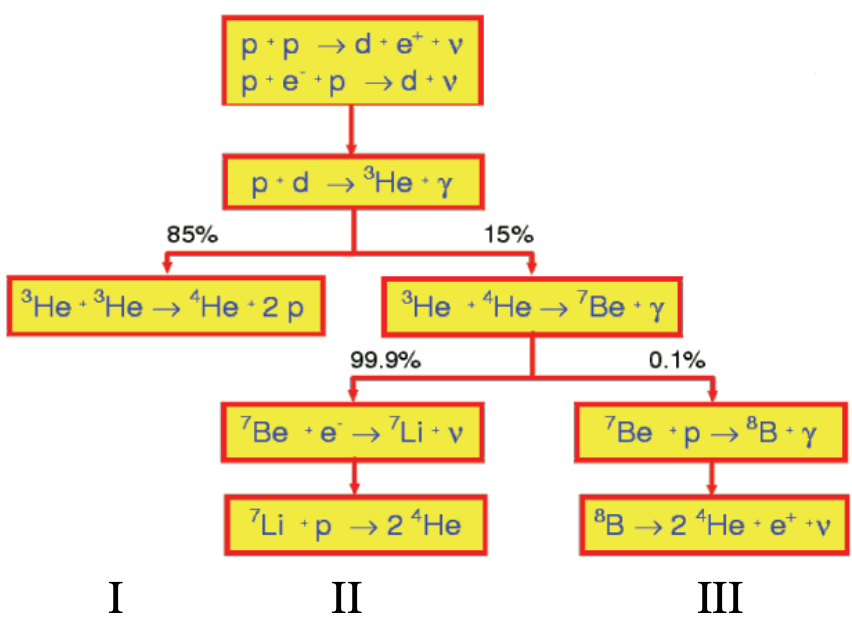
\includegraphics[width=9cm]{figures/figure2_1.png}
\captionsetup{justification=raggedright, singlelinecheck=false}
\caption{质子{}-{}质子链示意图。}
\label{ppchain}
\end{figure}

碳氮氧循环的路径则为
\begin{align*}
\ce{^{12}C}+\ce{^{1}H}&\to\ce{^{13}N}+\gamma,\\
\ce{^{13}N}&\to\ce{^{13}C}+\ce{e+}+\nu_{\ce{e}},\\
\ce{^{13}C}+\ce{^{1}H}&\to\ce{^{14}N}+\gamma,\\
\ce{^{14}N}+\ce{^{1}H}&\to\ce{^{15}O}+\gamma,\\
\ce{^{15}O}&\to\ce{^{15}N}+\ce{e+}+\nu_{\ce{e}},\\
\ce{^{15}N}+\ce{^{1}H}&\to\ce{^{12}C}+\ce{^{4}He}.
\end{align*}

温度高于$10^{8}\,\unit{K}$,将会进行氦燃烧:
\begin{align*}
\ce{^{4}He}+\ce{^{4}He}&\to\ce{^{8}Be},\\
\ce{^{8}Be}+\ce{^{4}He}&\to\ce{^{12}C}+\gamma.
\end{align*}

温度高于$\qty{5e8}{K}$时进行碳燃烧,共有五种路径:
\begin{align}
\ce{^{12}C}+\ce{^{12}C}&\to\ce{^{24}Mg}+\gamma,\notag\\
&\to\ce{^{23}Na}+\ce{p},\notag\\
&\to\ce{^{20}Ne}+\ce{^{4}He},\notag\\
&\to\ce{^{23}Mg}+\ce{n},\notag\\
&\to\ce{^{16}O}+2\ce{^{4}He}.\notag
\end{align}

温度高于$\qty{1.5e9}{K}$时进行氧燃烧
\begin{align}
\ce{^{16}O}+\ce{^{16}O}&\to\ce{^{32}S}+\gamma,\notag\\
&\to\ce{^{31}P}+\ce{p},\notag\\
&\to\ce{^{28}Si}+\ce{^{4}He},\notag\\
&\to\ce{^{31}S}+\ce{n},\notag\\
&\to\ce{^{24}Mg}+2\ce{^{4}He}.\notag
\end{align}

温度高于$\qty{3e9}{K}$时进行硅燃烧
\begin{align}
\ce{^{28}Si}+\ce{^{28}Si}&\to\ce{^{56}Ni}+\gamma,\notag\\
\ce{^{56}Ni}&\to\ce{^{56}Fe}+2\ce{e+}+2\nu_{\ce{e}}.\notag
\end{align}

更重元素的燃烧要求核心有更高的温度。热核反应导致恒星内部形成洋葱状结构,越里面的元素越重,温度越高。
\begin{figure}[!htbp]
\centering
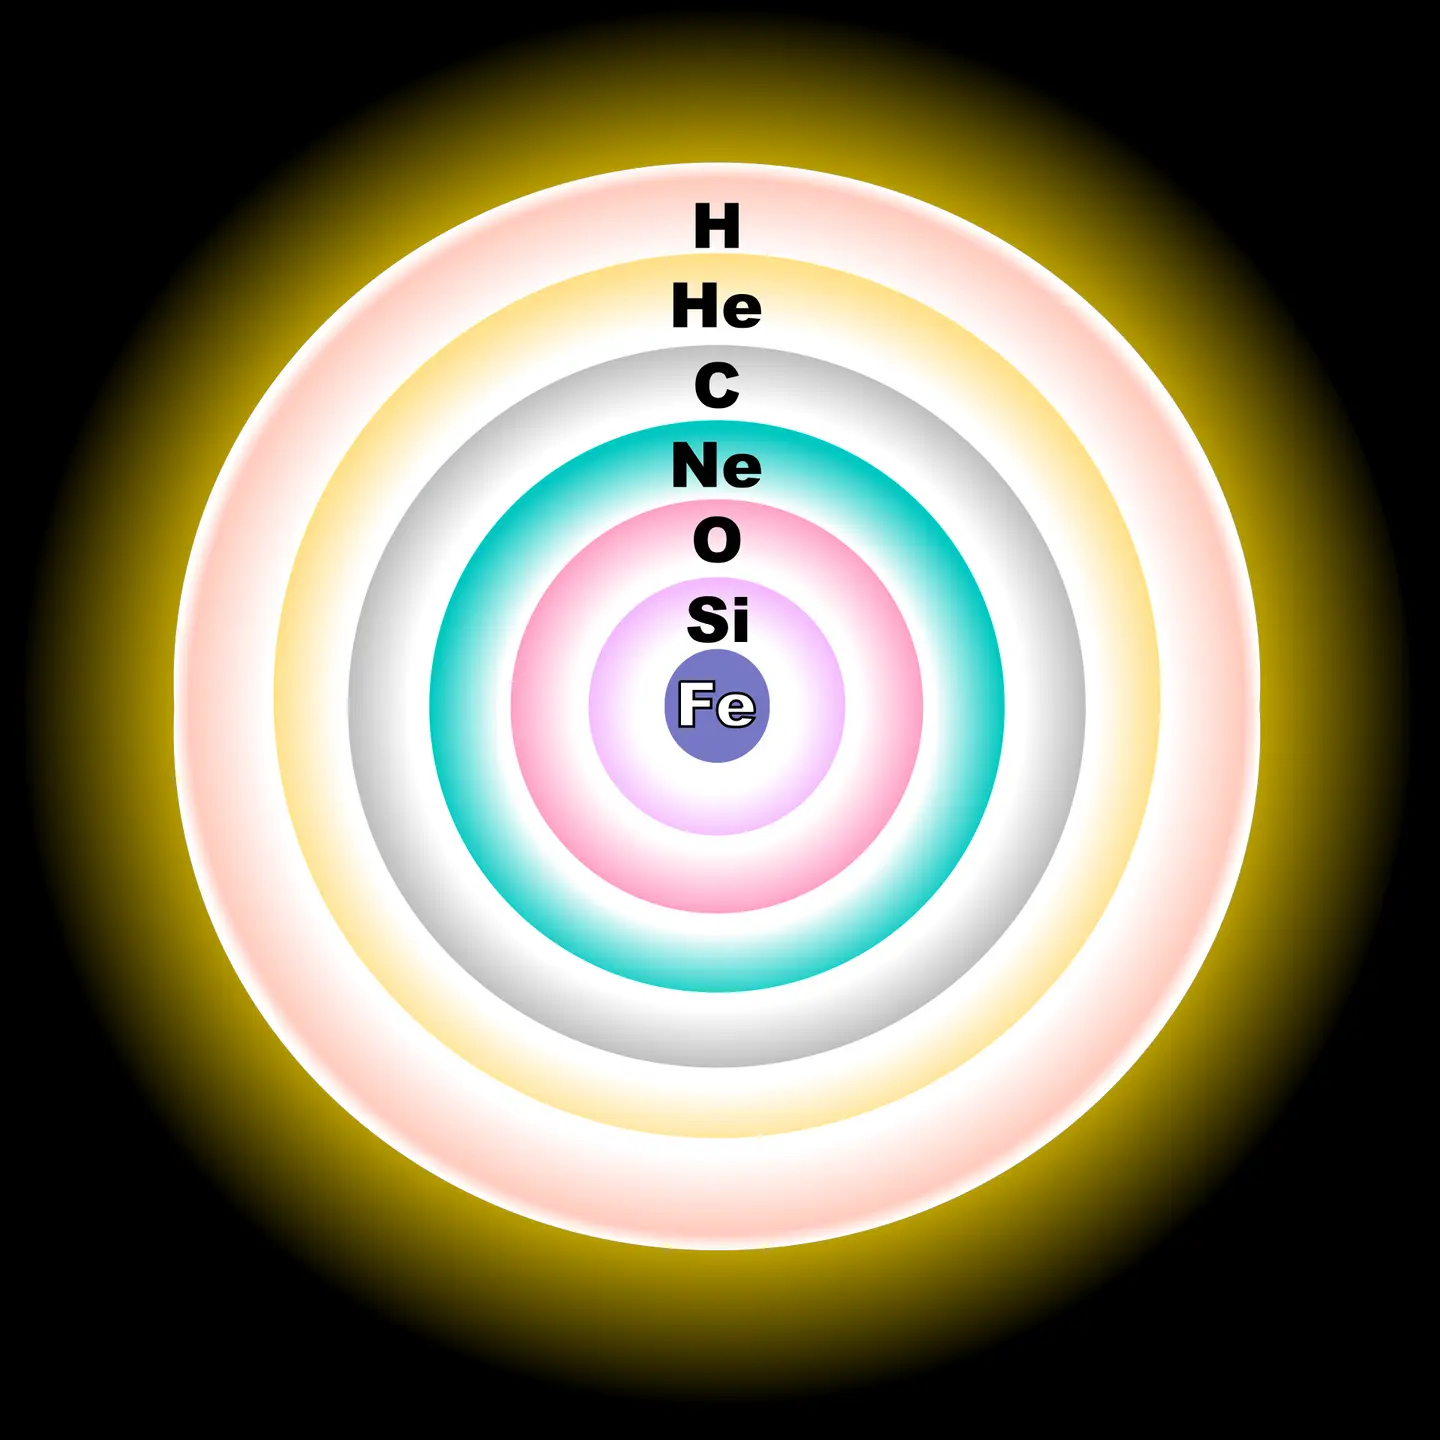
\includegraphics[width=7cm]{figures/figure2_2.JPG}
\captionsetup{justification=raggedright, singlelinecheck=false}
\caption{大质量恒星内部结构示意图。}
\label{大质量恒星内部结构示意图。}
\end{figure}

\subsubsection{能量传输和恒星振荡}
接下来我们研究能量在恒星内部的传输。首先建立能量守恒方程。记单位时间内通过半径为$r$的球面的能量为$L\left(r\right)$,单位物质在单位时间产生的能量(来自核反应和引力势能转换)为$\varepsilon\left(r\right)$,那么半径为$r$,厚度为$\mathrm{d}r$的球壳两侧的能量差为
\begin{equation}
\mathrm{d}L_{r}=L\left(r+\mathrm{d}r\right)-L\left(r\right)=\varepsilon\mathrm{d}M_{r}=4\pi{}r^{2}\rho\varepsilon\mathrm{d}r.
\end{equation}

恒星内部任意一点必须维持流体静力学平衡,而恒星内部核反应速率$\varepsilon$对温度十分敏感。温度上升势必导致反应速率上升,进而导致压强上升,强过小体元所受的引力,恒星核心区膨胀导致温度下降,形成负反馈,产生$\varepsilon$机制振荡。

能量传输有三种形式:辐射、传导和对流。太阳核心产生的能量主要通过辐射与对流 (convection) 向外传递。习惯上,我们用温度梯度来描述二者的贡献:
\begin{equation}
\frac{\mathrm{d}T}{\mathrm{d}r}=\left.\frac{\mathrm{d}T}{\mathrm{d}r}\right\vert{}_{\text{rad}}+\left.\frac{\mathrm{d}T}{\mathrm{d}r}\right\vert{}_{\text{conv}}.
\end{equation}

首先考虑辐射部分。其实我们已经推导过了,在介绍 Eddington 光度时就考虑过辐射压和引力的平衡,在推导质光关系时将其扩展得到
\begin{equation}
\frac{\mathrm{G}M}{r^{2}}=\frac{1}{\rho}\frac{\mathrm{d}P}{\mathrm{d}r}=\frac{1}{\mathrm{c}}\kappa\frac{L}{4\pi r^{2}}=\frac{1}{\rho}\frac{4}{3}a_{\text{B}}T^{3}\frac{\mathrm{d}T}{\mathrm{d}r},\tag{\ref{1.4.11}}
\end{equation}
稍作整理并修正下正负号便是所需要的方程
\begin{equation}
\frac{\mathrm{d}T}{\mathrm{d}r}=-\frac{3}{4a_{\text{B}}\mathrm{c}}\frac{\kappa\rho}{T^{3}}\frac{L_{r}}{4\pi r^{2}}.
\end{equation}
可见不透明度$\kappa$会影响辐射能传输的效率。不透明度下降,散逸的能量增多,导致核心区温度下降,压强下降,恒星收缩,密度上升,进而导致不透明度上升,产生$\kappa$机制振荡。

当恒星内部的不透明度或产能率增大时,辐射温度梯度值也随之增大,半径增加一点温度就快速下降,说明辐射不再是传递能量的有效方式,恒星依靠对流传递能量。或者当辐射平衡不稳定时,也会产生对流。对流是气体在冷热区域间大规模的循环流动。热气体膨胀上升,冷却后下沉,形成物质流动的循环和能量的传递。对流不仅传递能量,还起到混合物质的作用。

我们可以研究一下绝热条件下的温度梯度。假设恒星内部流体元在上升过程中绝热膨胀,不与周围交换热量,根据
\begin{equation}
P_{\text{g}}=\frac{\rho k_{\text{B}}T}{\mu m_{\ce{H}}}
\end{equation}
和
\begin{equation}
P=K\rho^{\gamma}
\end{equation}
可知
\begin{align}
\frac{\mathrm{d}P}{\mathrm{d}r}&=-\frac{P}{\mu}\frac{\mathrm{d}\mu}{\mathrm{d}r}+\frac{P}{\rho}\frac{\mathrm{d}\rho}{\mathrm{d}r}+\frac{P}{T}\frac{\mathrm{d}T}{\mathrm{d}r},\notag\\
\frac{\mathrm{d}P}{\mathrm{d}r}&=\gamma\frac{P}{\rho}\frac{\mathrm{d}\rho}{\mathrm{d}r},\notag\\
\left.\frac{\mathrm{d}T}{\mathrm{d}r}\right\vert{}_{\text{ad}}&=\left(1-\frac{1}{\gamma}\right)\frac{T}{P}\frac{\mathrm{d}P}{\mathrm{d}r}=-\left(1-\frac{1}{\gamma}\right)\frac{\mu m_{\ce{H}}}{k_{\text{B}}}\frac{\mathrm{G}M_{r}}{r^{2}}.
\end{align}
我们认为$\left\vert{}\dfrac{\mathrm{d}T}{\mathrm{d}r}\right\vert{}_{\text{actual}}<\left\vert{}\dfrac{\mathrm{d}T}{\mathrm{d}r}\right\vert{}_{\text{ad}}$的是辐射区,反之是对流区。

$M>1.5\text{\textendash}2\,\unit{M_{\odot}}$的恒星,拥有对流核区和辐射包层,核区发生$\ce{CNO}$循环核反应,产生能量的内核很小。

$0.8\,\unit{M_{\odot}}<M<1.5\text{\textendash}2\,\unit{M_{\odot}}$的恒星,拥有辐射核区和对流包层,核心区发生 pp chain 核反应,能量产生于较大的内核。

$0.1\,\unit{M_{\odot}}<M<0.8\,\unit{M_{\odot}}$的主序星,低温,整体对流。

\subsubsection{恒星的物态方程和气体总压强}
恒星内部的总压强主要由两部分组成:气体粒子运动产生的气体压强$P_{\text{g}}$和光子辐射压$P_{\text{rad}}$.不同的物态将会给出不同的压强形式。

对于非简并气体,我们在介绍质光关系的时候就计算过辐射压
\begin{equation}
P_{\text{rad}}=\frac{1}{3}a_{\text{B}}T^{4}.
\end{equation}
而对于气压,我们假设非简并气体状态方程为理想气体状态方程
\begin{equation}
P_{\text{g}}=nk_{B}T,
\end{equation}
其中$n$是粒子数密度。记气体一共包含$n'$摩尔的分子,那么
\begin{equation}
n=\frac{n'N_{\text{A}}}{V}=\frac{n'N_{\text{A}}}{\dfrac{m}{\rho}}=\frac{\rho}{\dfrac{m}{n'N_{\text{A}}}}=\frac{\rho}{\mu m_{\ce{H}}},
\end{equation}
其中$N_{\text{A}}$是阿伏伽德罗常数,$\mu$为平均相对分子质量,$m_{\ce{H}}$是质子的实际质量,数值上等于$\dfrac{1}{N_{\text{A}}}$.故非简并理想气体的气压可以写作
\begin{equation}
P_{\text{g}}=\frac{\rho k_{\text{B}}T}{\mu m_{\ce{H}}}.
\end{equation}
进一步,我们需要确定恒星中气体的相对分子量。考虑完全电离的中性等离子体,记$n_{i}$是各元素数密度,$\chi_{i}$是各元素所占的质量分数,$Z_{i}$是该元素的质子数(电荷数),$A_{i}$是该元素的质量数(即质子和中子数和),那么气压将是电子气体气压和各离子气体气压之和
\begin{equation}
P_{\text{g}}=n_{e}k_{\text{B}}T+\sum_{i}n_{i}k_{\text{B}}T=\sum_{i}\left(Z_{i}+1\right)n_{i}k_{\text{B}}T=\sum_{i}\left(1+Z_{i}\right)\frac{\rho\chi_{i}k_{\text{B}}T}{A_{i}m_{\ce{H}}}=\frac{\rho k_{\text{B}}T}{\mu m_{\ce{H}}}.
\end{equation}
因此相对分子量为
\begin{equation}
\frac{1}{\mu}=\sum_{i}\left(1+Z_{i}\right)\frac{\chi_{i}}{A_{i}}.
\end{equation}
习惯上记$\ce{H},\ce{He}$和金属元素的质量百分比为$X,Y,Z$,且认为金属元素质子数与中子数相当,即$\dfrac{Z_{i}}{A_{i}}=\dfrac{1}{2}$,那么对于考虑电子气体的情况,
\begin{equation}
P_{\text{g}}=\rho k_{\text{B}}T\frac{2X+\dfrac{3}{4}Y+\dfrac{1}{2}Z}{m_{\ce{H}}}.
\end{equation}

有时候我们不考虑电子气体的贡献,即只有一大堆离子,那么
\begin{align}
\frac{1}{\mu}&=\sum_{i}\frac{\chi_{i}}{A_{i}}\\
P_{\text{g}}&=\rho k_{\text{B}}T\frac{X+\dfrac{1}{4}Y}{m_{\ce{H}}}.
\end{align}
同时我们还能给出电子气体的相对分子质量来表征其贡献
\begin{equation}
\mu_{e}^{-1}=\sum_{i}\frac{Z_{i}\chi_{i}}{A_{i}}\approx X+\frac{1}{2}(1-X)=\frac{1+X}{2}.
\end{equation}

当引力越来越强时,即使密度不断提高,理想气体所提供的气压也不足以抗衡引力,此时电子简并压逐渐发挥主导作用。根据泡利不相容原理,电子不可能占据两个相同的能态,宏观上呈现出一定的抗压缩性。

\subsubsection{多方球模型}
结合边界条件:$r=0$时,$M\left(r\right)=0,L=0$; $r=R$时,$M\left(r\right)=M,T\left(r\right)=0,P\left(R\right)=0$.

恒星的多方球模型 (Polytropic Model).首先我们假设恒星是球对称结构,各物理量只与半径有关。其次,主序星处于完全流体静力学平衡,压强(来自气压和辐射压)梯度与引力平衡,得到
\begin{align}
\frac{\mathrm{G}M_{r}\rho\mathrm{d}A\mathrm{d}r}{r^{2}}&=\left(P\left(r\right)-P\left(r+\mathrm{d}r\right)\right)\mathrm{d}A=-\mathrm{d}P\left(r\right)\mathrm{d}A,\\
\frac{\mathrm{d}P}{\mathrm{d}r}&=-\frac{\mathrm{G}M_{r}\rho}{r^{2}}.\\
\frac{\mathrm{d}}{\mathrm{d}r}\left(\frac{r^{2}}{\rho}\frac{\mathrm{d}P}{\mathrm{d}r}\right)&=-\mathrm{G}\frac{\mathrm{d}M_{r}}{\mathrm{d}r}=-\mathrm{G}\left(4\pi r^{2}\rho\right).\\
\frac{1}{r^{2}}\frac{\mathrm{d}}{\mathrm{d}r}\left(\frac{r^{2}}{\rho}\frac{\mathrm{d}P}{\mathrm{d}r}\right)&=-4\pi{}\mathrm{G}\rho.
\end{align}
进一步假设恒星内部气体热量传输符合多方过程,即满足
\begin{equation}
P=K\rho^{1+\frac{1}{n}}=K\rho^{\gamma},
\end{equation}
如此一来压力引力平衡方程可以改写为
\begin{equation}
\left(\frac{n+1}{n}\right)\frac{K}{r^{2}}\frac{\mathrm{d}}{\mathrm{d}r}\left(r^{2}\rho^{\frac{1}{n}-1}\frac{\mathrm{d}\rho}{\mathrm{d}r}\right)=-4\pi\mathrm{G}\rho.\label{2.1.33}
\end{equation}
接着作代换
\begin{align}
\rho\left(r\right)&=\rho_{\text{c}}\left[\theta_{n}\left(r\right)\right]^{n},\\
r&=a_{n}\xi\left(r\right),\\
a_{n}&=\left[\frac{\left(n+1\right)K}{4\pi\mathrm{G}}\rho_{\text{c}}^{\frac{1}{n}-1}\right]^{\frac{1}{2}},
\end{align}
其中$\rho_{\text{c}}$代表恒星中心的密度,如此一来 (\ref{2.1.33}) 式可以改写为 Lane-Emden 方程的形式:
\begin{equation}
\frac{1}{\xi^{2}}\frac{\mathrm{d}}{\mathrm{d}\xi}\left(\xi^{2}\frac{\mathrm{d}\theta_{n}}{\mathrm{d}\xi}\right)=-\theta_{n}^{n}.
\end{equation}
上式仅在$n=0,1,5$时有解析解:
\begin{align}
\theta_{0}&=1-\frac{\xi^{2}}{6},\\
\theta_{1}&=\frac{\sin\xi}{\xi},\\
\theta_{5}&=\left[1+\frac{\xi^{2}}{3}\right]^{-\frac{1}{2}}.
\end{align}
其结果表明恒星从表面到中心密度、温度、压强等物理量是单调上升的。

\subsubsection{观测检验}
太阳对流区内的扰动在太阳内部产生各种形式的波动(日震波),表现为在太阳表面气体的起伏振荡(特征速度为几厘米/秒,周期约 5 分钟)和亮度变化。这种振荡可以通过太阳表面谱线的多普勒位移来测定。

由于振动频率可以精确测定,且频率依赖于恒星内部结构,恒星内部不同区域振荡模式不同,我们可以利用太阳的振荡现象研究太阳的内部结构。

中微子是一种不带电、质量极小的亚原子粒子,几乎不与任何物质相互作用。

太阳内部核聚变释放能量的$5\%$被中微子携带向外传输。

目前接收到的太阳的辐射实际上产生于$10^{5}\text{\textendash}10^{7}$年前的太阳内部,而中微子几乎产生于现在。

中微子会和四氯乙烯相互作用,生成半衰期$35$天的$\ce{Ar}$:
\begin{equation}
\ce{^{37}Cl}+\nu_{\ce{e}}\to\ce{^{37}Ar}+\ce{e-}.\\
\end{equation}
要进行反应$\nu_{\ce{e}}$能量最低达到$\qty{0.814}{MeV}$, 而$\ce{^{37}Ar}$的半衰期为 35 天。

也可以用纯水进行探测,中微子撞击电子将能量传递给电子后高速电子会产生切伦科夫辐射。

实际测量到的太阳中微子数目只有理论计算值的$\dfrac{1}{3}\text{\textendash}\dfrac{2}{3}$.

中微子在传播过程中发生了转换。太阳内部核反应只产生电子中微子,途中会产生$\mu$中微子和$\tau$中微子。表现为探测器白天黑夜得到的结果不一致(夜晚中微子穿过地球走的距离更长,转换得更多)。

1998 年日本超级神冈探测器通过测量大气中的$\mu$中微子变化,发现中微子振荡现象。

2001 年加拿大萨德伯里探测器测量到三种中微子,其中 35\%是电子中微子。

\subsection{恒星的演化}
恒星通过核反应产生能量,维持热平衡和流体静力学平衡。在此过程中恒星内部的化学组成发生变化。将新的化学组成作为初始条件重新代入方程组求解,得到恒星在时间$\mathrm{d}t$后的结构。依次类推,可以求得恒星的结构随时间的变化,即恒星的演化。

Russell-Vogt 原理:如果恒星处于流体静力学平衡和热平衡,而且它的能量来自内部的核反应,它们的结构和演化就完全唯一地由初始质量和化学丰度决定。

恒星的一生是与引力斗争的一生。

天文学中常用时标来估计某种物理过程的重要性,此处给出一些恒星演化中涉及的时标:

核时标,恒星核心区(约占总质量的$10\%$)核燃料消耗殆尽所需的时间
\begin{equation}
t_{n}=\frac{E}{L}=\frac{\eta\Delta{}M\mathrm{c}^{2}}{L}\approx0.7\%\times\frac{0.1\,M_{\odot}\mathrm{c}^{2}}{L}\approx10^{10}\,\unit{yr}\frac{M}{\unit{M_{\odot}}}\left(\frac{L}{\unit{L_{\odot}}}\right)^{-1}.
\end{equation}

热时标,恒星辐射完自身内能所需的时间,或者光子从恒星内部到达表面的时间(根据位力定理,内能是引力能的$\dfrac{1}{2}$)
\begin{equation}
t_{\text{the}}=0.5\frac{\mathrm{G}M^{2}}{RL}\approx2\times10^{7}\,\unit{yr}\left(\frac{M}{\unit{M_{\odot}}}\right)^{2}\left(\frac{R}{\unit{R_{\odot}}}\right)^{-1}\left(\frac{L}{\unit{L_{\odot}}}\right)^{-1}.
\end{equation}

动力学时标,如果恒星内部压力突然消失,引力作用下恒星坍缩的时间
\begin{equation}
t_{\text{dyn}}=\frac{R}{V}\approx\sqrt\frac{R^{3}}{\mathrm{G}M}\approx27\,\unit{min}\left(\frac{R}{\unit{R_{\odot}}}\right)^{\frac{3}{2}}\left(\frac{M}{\unit{M_{\odot}}}\right)^{-\frac{1}{2}}.
\end{equation}

\subsubsection{主序星演化}
随着核反应的进行,核心区的$\ce{H}$元素越来越少,直至枯竭,全部转变成$\ce{He}$.

主序带:主序星从核心$\ce{H}$燃烧开始到结束在赫罗图上占据的带状区域。

核反应$4\ce{^{1}H}\to\ce{^{4}He}$, 导致核心区粒子数下降,压强下降,核心收缩,温度上升,核反应产能率上升,光度上升,包层压力上升,恒星半径上升。

Schonberg-Chandrasekhar 质量极限:主序结束后在恒星核心形成一个等温氦核。氦核的内部压强必须能够支撑其上部包层物质的质量。

当恒星核心区的氢完全耗尽,恒星开始脱离主序。小质量、中等质量和大质量恒星主序后的演化路径差别很大。

大部分的$\ce{H,He}$和少部分的$\ce{Li,B,Be}$形成于宇宙大爆炸初期。

比$\ce{Fe}$轻的元素来自于恒星内部的核合成,比$\ce{Fe}$重的元素来自中子俘获反应。
\begin{align}
\left(Z,A\right)+\ce{n}&\to\left(Z,A+1\right)+\gamma,\\
\left(Z,A+1\right)&\to\left(Z+1,A+1\right)+\ce{e-}+\overline{\nu}_{\ce{e}}.
\end{align}
中子俘获反应有两种方式:慢中子俘获 (s-process) 和快中子俘获 (r-process).前者发生在中小质量恒星的渐近巨星支,后者发生在核坍缩超新星爆发和中子星并合。比如$\ce{^{26}Al}$只产生于核坍缩超新星爆发,半衰期为$\qty{7e5}{yr}$,衰变过程产生能量为$\qty{1.8}{Myr}$的$\gamma$射线,可追踪该辐射研究大质量恒星形成。

$\ce{^{26}Al}$只产生于核坍缩超新星爆发,它的半衰期只有$\qty{7e5}{yr}$.

中小质量恒星演化产生$\ce{C,N}$
大质量恒星演化产生$\ce{O}$
白矮星双星演化出$\ce{Fe}$

不同质量恒星演化主要区别:

演化过程不同:大质量恒星的内部碳可以点燃,形成更重的元素。

演化时标不同:大质量恒星的内部温度更高;主序星等寿命更短。

演化产物不同:大质量恒星通过超新星爆发,形成中子星或黑洞。

\begin{table}[!htbp]
\centering
\caption{不同质量恒星演化结局。}
\begin{tabular}{c c}
\hline
恒星初始质量$\left(\unit{M_{\odot}}\right)$ & 演化结局\\
\cline{1-2}
<0.01 & 行星\\
\cline{1-2}
0.01\text{\textendash}0.08 & 褐矮星\\
\cline{1-2}
0.08\text{\textendash}0.25 & $\rm He$白矮星\\
\cline{1-2}
0.25\text{\textendash}8 & $\rm CO$白矮星\\
\cline{1-2}
8\text{\textendash}10 & $\rm ONeMg$白矮星\\
\cline{1-2}
10\text{\textendash}20 & 超新星$\to$中子星\\
\cline{1-2}
>20 & 超新星$\to$黑洞\\
\hline
\end{tabular}
\label{}
\end{table}

\subsubsection{\texorpdfstring{$M\sim\qty{1}{M_{\odot}}$}{}恒星的主序后演化}

镜像原理:恒星处于壳层燃烧阶段时,恒星的核与包层相对该壳层作径向运动。即核收缩,包层扩张,核扩张,包层收缩。

随着表面温度的降低,$\ce{H-}$导致的不透明度增大,恒星对流区延伸到恒核心。林忠四郎线反映了(流体静力学)稳定的恒星在赫罗图上的边界。林忠四郎线左侧,对流和辐射可以有效传输能量。林忠四郎线右侧,没有任何机制可以有效传输能量

我们首先来介绍类太阳恒星的主序后演化。
\begin{table}[!htbp]
\centering
\caption{类太阳恒星的主序后演化过程。}
\begin{tabular}{c c c}
\hline
阶段 & 内部过程 & 赫罗图上的运动\\
\cline{1-3}
亚巨星支 & 核心区氢燃烧殆尽,氦核收缩 & 体积膨胀,表面温度降低,\\
(subgiant branch, SGB) & 壳层氢燃烧 & 恒星逐渐向右脱离主序\\
\cline{1-3}
红巨星支 & 氦核进一步收缩,核心压强上升, & 向右上方沿林忠四郎线\\
(red giant branch, RGB) & 温度上升,核区电子简并 & (Hayashi Track) 攀升成为红巨星\\
 & 壳层氢燃烧产能率上升,半径上升, & \\
 & 温度下降,恒星对流区增大 & \\
\cline{1-3}
氦闪 & $T_{\text{c}}$达到$10^{8}\,\unit{K}$时氦开始燃烧,& 攀升到红巨星支的顶点\\
(helium flash) & 由于电子简并,缺乏负反馈机制, & \\
 & 温度上升至氦爆燃,电子简并解除 & \\
\cline{1-3}
水平支 & 氦核燃烧,核心区半径上升,温度下降 & 向左下方移动至水平支\\
(horizontal branch, HB) & 壳层氢燃烧,壳层半径下降,温度上升 & \\
\cline{1-3}
渐近巨星支 & 氦核燃烧殆尽,留下$\mathrm{CO}$核,$R_{\text{c}}\downarrow,T_{\text{c}}\uparrow$ & 再次向右上方攀升\\
(asymptotic giant branch, AGB) & 壳层氢氦燃烧,壳层半径上升,温度下降 & 成为红超巨星\\
\cline{1-3}
热脉冲 & 壳层氦闪(不稳定燃烧),导致恒星脉动 & 移动到渐进巨星支顶端\\
(thermal pulse) & 红巨星包层物质抛射 ($25\text{\textendash}60\%$恒星质量) & \\
 & 形成行星状星云和高温简并$\mathrm{CO}$核 & \\
\cline{1-3}
白矮星 & 恒星外包层完全抛射,留下高温简并$\mathrm{CO}$核 & 向左下方移动至白矮星区\\
(white dwarf, WD) & 失去核反应,核心收缩,温度上升,靠简并压支撑 & \\
\hline
\end{tabular}
\label{}
\end{table}

行星状星云:低质量恒星在死亡时抛出的气体包层,受到中心高温白矮星的辐射电离而发光。通常为环形,年龄不超过五万年。

\subsubsection{\texorpdfstring{$M>\qty{2}{M_{\odot}}$}{}恒星的主序后演化}

恒星内部的$\ce{H}$燃烧通过$\mathrm{CNO}$循环进行,内部温度更高,辐射压对维持恒星的力学平衡起更大的作用,主序寿命更短。氦核不再简并。更重元素的燃烧可以平稳进行。核心区产生的能量主要以对流的方式向外传递。

\subsubsection{\texorpdfstring{$M>\qty{5}{M_{\odot}}$}{}恒星的主序后演化}

\begin{figure}[!htbp]
\centering
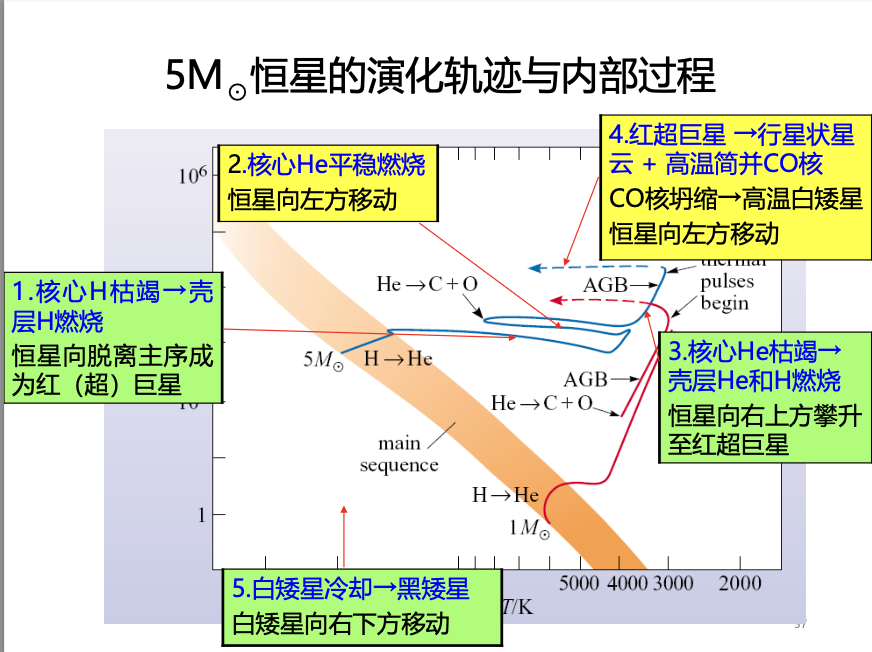
\includegraphics[width=10cm]{figures/figure2_6.png}
\captionsetup{justification=raggedright, singlelinecheck=false}
\caption{}
\label{}
\end{figure}

\subsubsection{\texorpdfstring{$M>\qty{8}{M_{\odot}}$}{}恒星的主序后演化}

观测表现为$\rm O$型星$\to$蓝超巨星$\to$黄超巨星$\to$红超巨星$\to$超新星。

\subsubsection{\texorpdfstring{$M>\qty{25}{M_{\odot}}$}{}恒星的主序后演化}

$\ce{O}$型星$\to$蓝超巨星$\to$红超巨星$\to$ WR 星$\to$ \uppercase\expandafter{\romannumeral1}b/\uppercase\expandafter{\romannumeral1}c 型超新星$\to$中子星/黑洞

高光度恒星通常有很强的星风(损失率$\sim10^{-6}\text{\textendash}10^{-4}\,\unit{M_{\odot}yr^{-1}}$),可以剥离恒星包层使氦核裸露。这类天体被称作沃尔夫{}-{}拉叶 (Wolf-Rayet, WR) 星。

\subsubsection{超新星爆发}

超新星爆发:核反应停止,核心区半径下降,温度上升,铁核氦核光致离解,产生电子俘获反应(电子和质子反应生成中子和中微子),电子密度下降,中微子带走能量,导致压强降低,星核坍缩,中子简并,核坍缩停止,形成中子星。包层物质下落,高速撞击导致激波反弹,壳层抛射,超新星爆发,形成致密星和超新星遗迹。其能量来源主要是包层物质引力能的释放。

不过即时爆发实际上是不可能的,因为激波中的绝大部分能量被用来离解下落的铁原子核,电子俘获过程产生的中微子带走了大部分能量。因此,需要给激波再次注入能量(如通过中微子与下落物质的相互作用),才能使爆发成功发生。

核坍缩超新星极大光度可达$10^{7}\text{\textendash}10^{10}\,\unit{L_{\odot}}$,总爆发能$10^{53}\,\unit{erg}$, 其中$99\%$以上以中微子形式释放;放射性衰变释放能量$\sim10^{49}\,\unit{erg}$, 可以产生时标几个月的可见光辐射;抛射物质$\sim10\,\unit{M_{\odot}}$, 速度$\sim\qty{3000}{km\cdot{}s^{-1}}$, 合计总动能$\sim10^{51}\,\unit{erg}$.

超新星遗迹:超新星爆发抛出的大量物质在向外膨胀过程中与星际物质和磁场相互作用而形成的气体星云。是强射电辐射和高能辐射源(同步加速辐射,激波加热)。年龄不超过十万年。

形态分类:壳层型,辐射主要来自纤维状的球形壳层和星际气体的相互作用;混合型,辐射来自遗迹整个区域,并且由中心的致密星提供能源。

按谱线有无氢线可将超新星爆发分为\uppercase\expandafter{\romannumeral1}型和\uppercase\expandafter{\romannumeral2}型。但同样是\uppercase\expandafter{\romannumeral1}型超新星,其没有氢线的原因也是不同的。

\uppercase\expandafter{\romannumeral1}a 型超新星源自双星系统中$\mathrm{CO}$白矮星吸积导致热核爆发,因此没有氢氦吸收线,有硅吸收线。爆发光变曲线陡峭,极大星等可达$-19$等。而\uppercase\expandafter{\romannumeral1}b 和\uppercase\expandafter{\romannumeral1}c 型超新星源自 WR 星的核坍缩,其中\uppercase\expandafter{\romannumeral 1}b 没有氢层有氦层,后者氢氦层都被剥离,因此\uppercase\expandafter{\romannumeral 1}b 型有弱氢、强氦吸收线,\uppercase\expandafter{\romannumeral 1}c 型没有氢氦吸收线,有弱硅吸收线。

\uppercase\expandafter{\romannumeral2}型超新星爆发源自超巨星的核坍缩。一个主序质量大于$\qty{8}{M_{\odot}}$,演化晚期质量大于$\qty{1.44}{M_{\odot}}$的星体,最后会发生电子俘获反应,让中微子带走大部分能量,核坍缩到中子简并,包层物质下落,引力能转化成动能产生激波反弹,壳层抛射$\alpha$元素(恒星元素合成主要是氦原子和其他原子碰撞,原子序数$+2+2$地增加),有核心和周围行星状星云残留。因为氢包层还存在,因此有氢吸收线,爆发后有一个持续几个月的平台期。\uppercase\expandafter{\romannumeral1}b, \uppercase\expandafter{\romannumeral1}c, \uppercase\expandafter{\romannumeral2}型超新星极大星等可达$-17\sim-16$等。

\uppercase\expandafter{\romannumeral 1}型超新星爆轰后什么也不会剩下,重金属元素会返还到星际介质中。而其他三种超新星有致密产物,如中子星或黑洞,重元素被锁在致密产物中。

宇宙早期,恒星形成剧烈且质量较大,金属丰度低,此时产生的超新星多是\uppercase\expandafter{\romannumeral 2}型超新星,$\alpha$元素增丰剧烈。就算有小质量恒星,\uppercase\expandafter{\romannumeral 1}型白矮星形成年龄$>\qty{40}{Myr}$,也要等到晚期。

等到薄盘形成之时,恒星形成率已显著降低,因此$\alpha$元素增丰显著放缓,而铁族元素由于\uppercase\expandafter{\romannumeral 1}a 超新星的贡献保持相对较快的增丰。

\uppercase\expandafter{\romannumeral1}型白矮星多存在于椭圆星系与旋涡星系,而其他三种超新星多存在于旋涡星系恒星形成区。

我们相信行星是从小尘埃一路碰撞聚合长成大行星的,一路碰下去能长很大的就比较少;而恒星是从一团很大的气体云坍缩的,坍缩成小团块的概率比较低;褐矮星就卡中间位置了,数量较少。

\subsubsection{观测检验}
恒星演化理论预言,热核反应是恒星的能源;恒星的主序寿命主要取决于初始质量;演化导致恒星脱离主序;恒星在不同演化阶段可观测的数目与在该阶段演化速度有关。

脉动变星 (Pulsating Variables) 是星体发生有节律的、大规模运动而使亮度发生变化的恒星。恒星演化到一定阶段,内部出现不稳定性,引力和压力失去平衡。维持脉动要求恒星在收缩时内部压力增大,在膨胀时内部压力减小。

经典造父变星的脉动周期越长,光度越高。质量$3\text{\textendash}10\,\unit{M_{\odot}}$的 F\text{\textendash}K 巨星,处于氦核燃烧阶段位于赫罗图主序上方的造父不稳定带。其光变主要来自表面温度的变化,半径越低,温度越高,光度又高。恒星演化到一定阶段,内部出现不稳定性,引力和压力失去平衡。维持脉动要求恒星在收缩时内部压力增大,在膨胀时内部压力减小。$\varepsilon$机制属于核心的核反应率变化。脉动主要是包层的周期性膨胀和收缩,不涉及恒星的核心。$\kappa$机制——包层不透明度的变化(阀门机制)。$\kappa\propto{}\rho{}T^{-3.5}$,一般情况下半径下降,导致温度上升,密度上升,$\kappa$减小,辐射更容易通过,包层失去能量,压力下降,半径进一步下降。但如果包层中有部分电离的元素($\ce{He+},\ce{He++}$),恒星收缩时部分对气体做的功会被用来进一步电离气体而不是提高温度,此时温度不变而密度上升,$\kappa$增大,辐射不易通过,包层吸收能量,压力上升,半径膨胀,形成负反馈。因此脉动的显著性(参与脉动的物质量、脉动振幅)等与部分电离区的位置有关。

\subsubsection{密近双星的演化}
1864 年,法国数学家$\rm E. Roche$首先提出计算密近双星系统引力势的简化模型。

方法:考虑在两个互相绕转的天体的引力势中一个检验粒子的运动

基本假设:

1. 每个子星的内部密度分布是球对称的,在动力学上可以认为是质点

2. 两子星以圆轨道绕公共质心运动

3. 两子星的自转和公转一致。

在以双星公共质心为原点的共转坐标系中,任意质点的欧拉方程是:
\begin{align}
\frac{\partial{}\boldsymbol{v}}{\partial{}t}&+\left(\boldsymbol{v}\cdot\nabla\right)\boldsymbol{v}=-\nabla\Phi-2\boldsymbol{\omega}\times\boldsymbol{v}-\frac{1}{\rho}\nabla P,\notag\\
\Phi\left(r\right)&=-\frac{\mathrm{G}M_{1}}{\left\vert{}\boldsymbol{r}-\boldsymbol{r}_{1}\right\vert{}}-\frac{\mathrm{G}M_{2}}{\left\vert{}\boldsymbol{r}-\boldsymbol{r}_{2}\right\vert{}}-\frac{1}{2}\left(\boldsymbol{\omega}\times\boldsymbol{r}\right)^{2}.
\end{align}

临界等势面:同时包络两颗子星并且相接于其间一点 (L1) 的等势面。


洛希瓣:由临界等势面包围的空间。

在$\rm L_1$点,两颗子星对物质产生的作用力正好相等,$\rm Roche$势达极大值

当子星充满洛希瓣后,在内拉格朗日附近的物质处于不稳定状态,受到小扰动就会流向伴星,产生物质交流。


根据双星中的一颗或两颗子星是否充满洛希瓣,可以将双星分为

不相接双星 (detached binaries): 两颗子星均未充满洛希瓣。
半相接双星 (semidetached binaries):一颗子星充满洛希瓣,如天琴座β。

相接双星 (contact binaries):两颗子星均充满洛希瓣,如大熊座 W。

双星间的物质传输:

1. 星风俘获(不相接、半相接):恒星星风中的部分物质被伴星引力俘获

2. 洛希瓣渗溢(半相接、相接):充满洛希瓣的恒星的大气通过 L1 流向伴星,并在其周围生成吸积盘。

大陵佯谬:大陵五主星是一颗质量$\qty{3.7}{M_{\odot}}$的主序星,伴星是一颗质量$\qty{0.8}{M_{\odot}}$的亚巨星。为什么质量小的恒星反而演化得快?



行星状星云的形成:双星轨道运动改变星云形态。吸积/抛射过程产生双极结构。

蓝离散星 (Blue Stragglers) 的形成:星团中比脱离主序点处的恒星更蓝、更亮的恒星。形成机制:双星的碰撞并合、物质传输。


\begin{table}[!htbp]
\centering
\caption{致密星能源与辐射}
\begin{tabular}{c c c}
\hline
能源 & 物理过程 & 观测表现\\
\cline{1-3}
内能 & 冷却 & 白矮星的紫外、光学辐射,中子星的软 X 射线辐射\\
\cline{1-3}
转动动能 & 自转减慢 & 射电脉冲星,各种喷流\\
\cline{1-3}
磁能 & 磁场的耗散与重组 & 强磁星\\
\cline{1-3}
引力势能 & 物质吸积 & 激变变星(白矮星),X 射线双星,中子星,黑洞\\
\cline{1-3}
核能 & 表面热核反应 & 新星爆发(白矮星)、\uppercase\expandafter{\romannumeral1}型 X 射线爆发(中子星)\\
\hline
\end{tabular}
\label{}
\end{table}


\subsection{白矮星}
白矮星内部高温高密,高温使原子电离产生大量自由电子,高密使电子简并产生电子简并压。

白矮星基本参数:
质量$\sim0.2\text{\textendash}1.3\,\unit{M_{\odot}}$, 半径$\sim5\times10^{8}\text{\textendash}10^{9}\,\unit{cm}$, 密度$\sim10^{5}\text{\textendash}10^{7}\,\unit{g\cdot cm^{-3}}$, 绝对星等$M_{\text{V}}\sim8\text{\textendash}16$, 有效温度$\sim5\times10^{3}\text{\textendash}4\times10^{4}\,\unit{K}$,自转周期$\ge\qty{10}{s}$. 外层包裹着厚度约$\qty{50}{km}$,主要由氢组成的大气。

对于非相对论性 ($v_{e}\ll c$) 电子,$P_{e}\propto\rho^{\frac{5}{3}}$,对于相对论性电子,$P_{e}\propto\rho^{\frac{4}{3}}$.

随着白矮星质量增大,白矮星质量增大,简并气体运动变成相对论性。此时引力$\dfrac{\mathrm{G}\rho{}M}{R^{2}}\propto{}\dfrac{M^{2}}{R^{5}}$比压力$\dfrac{\mathrm{d}P}{\mathrm{d}R}\propto{}\dfrac{\rho^{\frac{4}{3}}}{R}\propto{}\dfrac{M^{\frac{4}{3}}}{R^{5}}$增长得更快,因此白矮星有质量上限。

白矮星冷却产生光学、紫外辐射。由于热传导的效率很高,白矮星内部几乎是等温的。

激变变星是白矮星与低质量恒星构成的半相接双星,白矮星吸积伴星物质,表面发生失控的热核反应,产生光学、紫外、X 射线辐射和爆发,同时抛射吸积物质。激变变星有新星、再发新星等分类。

新星的观测特征为在数天至数星期内亮度增加$7\text{\textendash}16$等,然后缓慢下降,经几个月或几年回复到原先的状态。辐射主要在光学和紫外波段,爆发时的能量释放率$\sim10^{45}\text{\textendash}10^{46}\,\unit{erg\cdot{}s^{-1}}$,抛射约$10^{-5}\text{\textendash}10^{-3}\,\unit{M_{\odot}}$的物质。

物质传输会导致新星反复爆发,表现为再发新星,爆发间隔约$10\text{\textendash}100$年。

等总质量达到钱德拉塞卡质量极限时转变为\uppercase\expandafter{\romannumeral1}a 型超新星,光变在爆发后 20 天达到峰值,接着在一个月左右的时间内快速下降$\ce{^{56}Ni}$衰变,然后缓慢下降$\ce{^{56}Co}$衰变。

M。菲利普发现 B 波段峰值星等与峰值后 15 天星等的衰减量有很好的相关性。光度衰减得越快,峰值光度越低。利用该关系将光变曲线归一化后,\uppercase\expandafter{\romannumeral1}a 型超新星几乎具有相同的峰值光度,是已知最好的标准烛光源。

\subsection{中子星}

白矮星质量超过钱德拉塞卡极限时,电子简并压不足以抵抗引力。原子核开始瓦解,依靠中子简并压抵抗引力。中子星可以看作是一个巨型原子核,由$\sim10^{57}$个中子构成。

中子星的特征质量为$\qty{1.4}{M_{\odot}}$,半径约$\qty{10}{km}$.

中子星的观测表现:内能表现为热辐射。转动动能表现为脉冲星。强引力场表现为 X 射线双星。强磁场表现为强磁星。

为什么脉冲星是中子星?

首先脉冲持续时间很短,小于$\qty{100}{ms}$,说明辐射源大小也小于$\qty{3e9}{cm}$.

脉冲周期不变,不可能出于能量会损耗的双星轨道运动;脉冲周期远快于形体脉动;脉冲周期快于白矮星自转。因此脉冲星只能是中子星。

脉冲星的能量来源和辐射机制是什么?


X 射线双星:吸积物质的引力势能转化为动能,进而转化为热能,温度高达$10^{7}\,\unit{K}$,表现为 X 射线辐射。根据伴星质量不同分为两类。高质量$M>\qty{10}{M_{\odot}}$ X 射线双星,伴星早型,质量大,年轻$<10^{7}\,\unit{yr}$,分布在银盘附近,中子星具有强磁场,物质来自星风。低质量$M\le\qty{1}{M_{\odot}}$ X 射线双星,伴星晚型,低质量,年老$>\qty{5e9}{yr}$,物质来自洛希瓣渗溢,分布在银心和球状星团中,中子星具有弱磁场。

在高质量 X 射线双星中,吸积流在中子星磁层处被截断。吸积物质沿着中子星磁力线流向中子星的两极。由此产生的辐射是非各向同性的,表现为 X 射线脉冲星。

低质量 X 射线双星往往具有 X 射线暴。上升时标$\sim1\text{\textendash}10\,\unit{s}$,衰减时标数十秒,释放能量$10^{39}\text{\textendash}10^{40}\,\unit{erg}$,爆发间隔几小时,爆发机制吸积中子星表面 H, He 壳层的失控热核反应。

\subsection{黑洞}
描述黑洞的物理参数只有质量、角动量和电荷。

黑洞的分类

只由质量来表征的球对称、静态的史瓦西黑洞;

球对称、静态的、带电的莱斯纳{}-{}诺德斯特洛姆黑洞;

转动且电中性的克尔黑洞;

转动且带电的克尔{}-{}纽曼黑洞。

\subsubsection{Schwarzschild}
视界:半径为史瓦西半径$R_{\text{s}}$的球面,在视界内的任何信息都无法向外传递

光层:半径为$1.5R_{\text{s}}$的球面,在光层各向同性辐射光子中的一半可以逃逸

\subsubsection{Kerr}
对角动量为$J$的黑洞,记$m=\dfrac{\mathrm{G}M}{\mathrm{c}^{2}},a=\dfrac{J}{M\mathrm{c}}$,视界半径为
\begin{equation}
r_{\text{h}}=\left(\frac{R_{\text{s}}}{2}\right)\left[m+\sqrt{m^{2}-a^{2}}\right].
\end{equation}
能层为
\begin{equation}
r_{\text{st}}=\left(\frac{R_{\text{s}}}2\right)\left[m+\sqrt{m^{2}-a^{2}\cos^{2}\theta}\right].
\end{equation}
能层:介于$r_{\text{h}}$和$r_{\text{st}}$之间的区域。

由于引力透镜效应,黑洞阴影的半径为
\begin{equation}
R_{\text{shadow}}=\frac{\sqrt{27}\mathrm{G}M}{\mathrm{c}^{2}}.
\end{equation}

广义相对论预言处于转动状态的质量会拖拽周围的时空。黑洞能层内的时空必须同它一起转动。

黑洞蒸发具有黑体辐射的特征。

黑洞视界面的温度:
\begin{equation}
kT\sim\frac{h\mathrm{c}}{\lambda}=\frac{h\mathrm{c}}{2\mathrm{G}M/\mathrm{c}^{2}}=\frac{h\mathrm{c}^{3}}{2\mathrm{G}M},
\end{equation}
根据黑洞能损率推测黑洞寿命
\begin{equation}
t=\frac{E}{L}=\frac{M\mathrm{c}^{2}}{4\pi R_{\text{s}}^{2}\sigma T^{4}}\propto{}M^{3}
\end{equation}

$M=\qty{1}{M_{\odot}},T\sim10^{-6}\,\unit{K},t\sim10^{67}\,\unit{yr}$,

$M=10^{15}\,\unit{g},T\sim10^{13}\,\unit{K},t\sim10^{10}\,\unit{yr}$.因此小黑洞已经蒸发。

\subsubsection{如何搜索黑洞?}
黑洞强引力场的观测效应:

黑洞附近的光线偏折和红移;

黑洞的物质吸积过程;

黑洞并合产生的引力波。

恒星级吸积黑洞靠黑洞 X 射线双星,搜寻质量超过中子星质量上限的致密天体,确定其性质(X 射线辐射、时变)、轨道运动和质量。

微类星体 (microquasars):具有相对论性喷流的黑洞 X 射线双星。


\subsection{行星}
假设行星是黑体,能量全部来自太阳,得到
\begin{equation}
\frac{L_{\odot}}{4\pi R^{2}_{\odot\to\text{planet}}}\pi R_{\text{planet}}^{2}\times\left(1-a\right)=4\pi R_{\text{planet}}^{2}\sigma_{\text{SB}}T_{\text{planet}}^{4}.
\end{equation}
可借此估计行星温度,其中$a$是反照率。

\printbibliography
\end{document}